\documentclass{ximera}
\graphicspath{  %% When looking for images,
{./}            %% look here first,
{./pictures/}   %% then look for a pictures folder,
{../pictures/}  %% which may be a directory up.
{../../pictures/}  %% which may be a directory up.
{../../../pictures/}  %% which may be a directory up.
{../../../../pictures/}  %% which may be a directory up.
}

\usepackage{listings}
%\usepackage{circuitikz}
\usepackage{xcolor}
\usepackage{amsmath,amsthm}
\usepackage{subcaption}
\usepackage{graphicx}
\usepackage{tikz}
%\usepackage{tikz-3dplot}
\usepackage{amsfonts}
%\usepackage{mdframed} % For framing content
%\usepackage{tikz-cd}

  \renewcommand{\vector}[1]{\left\langle #1\right\rangle}
  \newcommand{\arrowvec}[1]{{\overset{\rightharpoonup}{#1}}}
  \newcommand{\ro}{\texttt{R}}%% row operation
  \newcommand{\dotp}{\bullet}%% dot product
  \renewcommand{\l}{\ell}
  \let\defaultAnswerFormat\answerFormatBoxed
  \usetikzlibrary{calc,bending}
  \tikzset{>=stealth}
  




%make a maroon color
\definecolor{maroon}{RGB}{128,0,0}
%make a dark blue color
\definecolor{darkblue}{RGB}{0,0,139}
%define the color fourier0 to be the maroon color
\definecolor{fourier0}{RGB}{128,0,0}
%define the color fourier1 to be the dark blue color
\definecolor{fourier1}{RGB}{0,0,139}
%define the color fourier 1t to be the light blue color
\definecolor{fourier1t}{RGB}{173,216,230}
%define the color fourier2 to be the dark green color
\definecolor{fourier2}{RGB}{0,100,0}
%define teh color fourier2t to be the light green color
\definecolor{fourier2t}{RGB}{144,238,144}
%define the color fourier3 to be the dark purple color
\definecolor{fourier3}{RGB}{128,0,128}
%define the color fourier3t to be the light purple color
\definecolor{fourier3t}{RGB}{221,160,221}
%define the color fourier0t to be the red color
\definecolor{fourier0t}{RGB}{255,0,0}
%define the color fourier4 to be the orange color
\definecolor{fourier4}{RGB}{255,165,0}
%define the color fourier4t to be the darker orange color
\definecolor{fourier4t}{RGB}{255,215,0}
%define the color fourier5 to be the yellow color
\definecolor{fourier5}{RGB}{255,255,0}
%define the color fourier5t to be the darker yellow color
\definecolor{fourier5t}{RGB}{255,255,100}
%define the color fourier6 to be the green color
\definecolor{fourier6}{RGB}{0,128,0}
%define the color fourier6t to be the darker green color
\definecolor{fourier6t}{RGB}{0,255,0}

%New commands for this doc for errors in copying
\newcommand{\eigenvar}{\lambda}
%\newcommand{\vect}[1]{\mathbf{#1}}
\renewcommand{\th}{^{\text{th}}}
\newcommand{\st}{^{\text{st}}}
\newcommand{\nd}{^{\text{nd}}}
\newcommand{\rd}{^{\text{rd}}}
\newcommand{\paren}[1]{\left(#1\right)}
\newcommand{\abs}[1]{\left|#1\right|}
\newcommand{\R}{\mathbb{R}}
\newcommand{\C}{\mathbb{C}}
\newcommand{\Hilb}{\mathbb{H}}
\newcommand{\qq}[1]{\text{#1}}
\newcommand{\Z}{\mathbb{Z}}
\newcommand{\N}{\mathbb{N}}
\newcommand{\q}[1]{\text{``#1''}}
%\newcommand{\mat}[1]{\begin{bmatrix}#1\end{bmatrix}}
\newcommand{\rref}{\text{reduced row echelon form}}
\newcommand{\ef}{\text{echelon form}}
\newcommand{\ohm}{\Omega}
\newcommand{\volt}{\text{V}}
\newcommand{\amp}{\text{A}}
\newcommand{\Seq}{\textbf{Seq}}
\newcommand{\Poly}{\textbf{P}}
\renewcommand{\quad}{\text{    }}
\newcommand{\roweq}{\simeq}
\newcommand{\rowop}{\simeq}
\newcommand{\rowswap}{\leftrightarrow}
\newcommand{\Mat}{\textbf{M}}
\newcommand{\Func}{\textbf{Func}}
\newcommand{\Hw}{\textbf{Hamming weight}}
\newcommand{\Hd}{\textbf{Hamming distance}}
\newcommand{\rank}{\text{rank}}
\newcommand{\longvect}[1]{\overrightarrow{#1}}
% Define the circled command
\newcommand{\circled}[1]{%
  \tikz[baseline=(char.base)]{
    \node[shape=circle,draw,inner sep=2pt,red,fill=red!20,text=black] (char) {#1};}%
}

% Define custom command \strikeh that just puts red text on the 2nd argument
\newcommand{\strikeh}[2]{\textcolor{red}{#2}}

% Define custom command \strikev that just puts red text on the 2nd argument
\newcommand{\strikev}[2]{\textcolor{red}{#2}}

%more new commands for this doc for errors in copying
\newcommand{\SI}{\text{SI}}
\newcommand{\kg}{\text{kg}}
\newcommand{\m}{\text{m}}
\newcommand{\s}{\text{s}}
\newcommand{\norm}[1]{\left\|#1\right\|}
\newcommand{\col}{\text{col}}
\newcommand{\sspan}{\text{span}}
\newcommand{\proj}{\text{proj}}
\newcommand{\set}[1]{\left\{#1\right\}}
\newcommand{\degC}{^\circ\text{C}}
\newcommand{\centroid}[1]{\overline{#1}}
\newcommand{\dotprod}{\boldsymbol{\cdot}}
%\newcommand{\coord}[1]{\begin{bmatrix}#1\end{bmatrix}}
\newcommand{\iprod}[1]{\langle #1 \rangle}
\newcommand{\adjoint}{^{*}}
\newcommand{\conjugate}[1]{\overline{#1}}
\newcommand{\eigenvarA}{\lambda}
\newcommand{\eigenvarB}{\mu}
\newcommand{\orth}{\perp}
\newcommand{\bigbracket}[1]{\left[#1\right]}
\newcommand{\textiff}{\text{ if and only if }}
\newcommand{\adj}{\text{adj}}
\newcommand{\ijth}{\emph{ij}^\text{th}}
\newcommand{\minor}[2]{M_{#2}}
\newcommand{\cofactor}{\text{C}}
\newcommand{\shift}{\textbf{shift}}
\newcommand{\startmat}[1]{
  \left[\begin{array}{#1}
}
\newcommand{\stopmat}{\end{array}\right]}
%a command to give a name to explorations and hints and theorems
\newcommand{\name}[1]{\begin{centering}\textbf{#1}\end{centering}}
\newcommand{\vect}[1]{\vec{#1}}
\newcommand{\dfn}[1]{\textbf{#1}}
\newcommand{\transpose}{\mathsf{T}}
\newcommand{\mtlb}[2][black]{\texttt{\textcolor{#1}{#2}}}
\newcommand{\RR}{\mathbb{R}} % Real numbers
\newcommand{\id}{\text{id}}
\newcommand{\coord}[1]{\langle#1\rangle}
\newcommand{\RREF}{\text{RREF}}
\newcommand{\Null}{\text{Null}}
\newcommand{\Nullity}{\text{Nullity}}
\newcommand{\Rank}{\text{Rank}}
\newcommand{\Col}{\text{Col}}
\newcommand{\Ef}{\text{EF}}
\newcommand{\boxprod}[3]{\abs{(#1\times#2)\cdot#3}}

\author{Zack Reed}
%borrowed from selinger linear algebra
\begin{document}


\begin{problem}
  Consider the following collection of points in $\R^2$:
  \begin{equation*}
    \set{
      \startmat{r} 1 \\ -1 \stopmat,
      \startmat{r} -2 \\ 1 \stopmat,
      \startmat{r} 3 \\ -2 \stopmat,
      \startmat{r} 2 \\ -2 \stopmat,
      \startmat{r} -2 \\ 1 \stopmat,
      \startmat{r} 3 \\ -1 \stopmat,
      \startmat{r} -3 \\ 0 \stopmat,
      \startmat{r} 0 \\ 3 \stopmat,
      \startmat{r} 0 \\ 0 \stopmat,
      \startmat{r} 0 \\ -2 \stopmat
    }.
  \end{equation*}
  Find the 1-dimensional subspace that best approximates this
  collection of points. What is the total squared lengths of the projections onto this subspace? What is the total squared distance of the
  points to the subspace? 

  \begin{solution}
  
    The best-fitting $1D$ subspace is $\span\left(\begin{bmatrix}
      \answer[tolerance=.01]{-.832}\\\answer[tolerance=.01]{.554}
    \end{bmatrix}\right)$. (Note: the vector should be a unit vector with a negative first coordinate rounded to four decimal places.)

    The total squared lengths of the projections onto the subspace is $\answer[tolerance=.5]{52}$. (Hint: Remember that the singular values $\sigma$ capture the norm $\norm{A\vec{v}_1}$, the square root of the dot product of the data with the right singular vector $\vec{v}_1$.)

    The total squared distance of the points to the subspace is $\answer[tolerance=.5]{13}$ (Hint: The singular vectors not spanning the best-fit subspace form basis vectors for $\RR^m$ outside of the best-fit subspace, and the remaining singular values account for the spread along those directions.)

  \end{solution}


\end{problem}

\begin{problem}
  Consider the following collection of points in $\R^3$. Do not assume this has been centered on the origin, plot the points to determine this.
  \begin{equation*}
    \set{
      \startmat{r} 0 \\ 0 \\ 9 \stopmat,
      \startmat{r} 1 \\ 0 \\ -3 \stopmat,
      \startmat{r} 0 \\ 0 \\ 1 \stopmat,
      \startmat{r} 0 \\ 5 \\ -4 \stopmat,
      \startmat{r} 6 \\ -2 \\ 13 \stopmat,
      \startmat{r} 1 \\ 0 \\ 0 \stopmat,
      \startmat{r} 0 \\ 2 \\ 0 \stopmat,
      \startmat{r} 0 \\ 1 \\ 1 \stopmat,
      \startmat{r} 2 \\ 0 \\ 0 \stopmat,
      \startmat{r} 4 \\ 0 \\ 0 \stopmat,
      \startmat{r} 1 \\ -3 \\ 0 \stopmat,
      \startmat{r} 0 \\ 0 \\ 4 \stopmat
    }.
  \end{equation*}
  \begin{enumerate}
  \item Find the 1-dimensional subspace that best approximates this
    collection of points.
  \item Find the 2-dimensional subspace that best approximates this
    collection of points.
  \end{enumerate}
  In each case, what is the total squared distance of the points to
  the subspace? What is the total length of the projections of the points onto the subspace.

  \begin{solution}
    
    \begin{enumerate}
      \item The best-fitting $1D$ subspace is $\span\left(\begin{bmatrix}
        \answer[tolerance=.005]{.2120}\\\answer[tolerance=.005]{-.2192}\\\answer[tolerance=.005]{.9524}
      \end{bmatrix}\right)$ (The direction vector is a unit vector, the first coordinate is positive. Round to four decimal places.)

      The total squared distance of the points to the subspace is $\answer{60}$ (Round to the nearest integer).

      The total spread (i.e. the total squared proejction lengths) is $\answer[tolerance=1]{279}$ (Round to the nearest integer).

      \item The best-fitting $2D$ subspace is $\span\left(\begin{bmatrix}
        \answer[tolerance=.005]{.2120}\\\answer[tolerance=.005]{-.2192}\\\answer[tolerance=.005]{.9524}
      \end{bmatrix},\begin{bmatrix}
        \answer[tolerance=.005]{.6434}\\\answer[tolerance=.005]{-.7022}\\\answer[tolerance=.005]{-.3049}
      \end{bmatrix}\right)$ (The direction vectors are unit vectors, the first coordinate of both vectors is positive. Round to four decimal places.)

      The total squared distance of the points to the subspace is $\answer{22}$ (Round to the nearest integer).

      The total spread (i.e. the total squared proejction lengths) is $\answer[tolerance=1]{316}$ (Round to the nearest integer).
    \end{enumerate}

  \end{solution}

\end{problem}

%\begin{problem}
%  Find the principal components of the matrix
%  \begin{equation*}
%    A = \startmat{ccccccccc}
%      0 & 0 & 0 & 0 & -1 & 0 & 3 & 0 & 1 \\
%      0 & 1 & 0 & 0 & 2 & 3 & 0 & 2 & -1 \\
%      1 & -1 & -3 & 3 & -1 & 0 & 0 & -2 & 2 \\
%    \stopmat.
%  \end{equation*}
%\end{problem}

%\begin{problem}
 % Compute the centroid of the following collection of points:
 % \begin{equation*}
 %   \set{
 %     \startmat{r} 2 \\ -1 \stopmat,
 %     \startmat{r} 0 \\ 1 \stopmat,
 %     \startmat{r} 4 \\ -3 \stopmat,
 %     \startmat{r} -4 \\ -4 \stopmat,
 %     \startmat{r} 0 \\ -2 \stopmat,
 %     \startmat{r} -2 \\ -1 \stopmat,
 %     \startmat{r} 0 \\ -2 \stopmat,
 %     \startmat{r} -2 \\ -4 \stopmat,
 %     \startmat{r} 3 \\ -1 \stopmat,
 %     \startmat{r} -5 \\ -5 \stopmat
 %   }.
 % \end{equation*}
%\end{problem}

%\begin{problem}
%  Consider the following collection of points in $\R^2$:
%  \begin{equation*}
%    \set{
%      \startmat{r} 4 \\ -3 \stopmat,
%      \startmat{r} 10 \\ -9 \stopmat,
%      \startmat{r} 4 \\ -7 \stopmat,
%      \startmat{r} -2 \\ 3 \stopmat,
%      \startmat{r} 10 \\ -3 \stopmat,
%      \startmat{r} 4 \\ -3 \stopmat,
%      \startmat{r} 5 \\ -3 \stopmat,
%      \startmat{r} 4 \\ 1 \stopmat,
%      \startmat{r} -2 \\ -3 \stopmat,
%      \startmat{r} 3 \\ -3 \stopmat
%    }.
%  \end{equation*}
%  Compute the centroid, and then find the 1-dimensional affine
%  subspace that best approximates this collection of points. What is
%  the total squared distance of the points to the subspace?
%\end{problem}

\begin{problem}
  Consider the following collection of points in $\R^3$:
  \begin{equation*}\scriptstyle
    \set{
      \startmat{r} 0 \\ -2 \\ 2 \stopmat,
      \startmat{r} 6 \\ 2 \\ 2 \stopmat,
      \startmat{r} 2 \\ 2 \\ 6 \stopmat,
      \startmat{r} 3 \\ 2 \\ 2 \stopmat,
      \startmat{r} 3 \\ 0 \\ 5 \stopmat,
      \startmat{r} 5 \\ 0 \\ 2 \stopmat,
      \startmat{r} 4 \\ -2 \\ -2 \stopmat,
      \startmat{r} 5 \\ 0 \\ 2 \stopmat,
      \startmat{r} 1 \\ 0 \\ 2 \stopmat,
      \startmat{r} 3 \\ 0 \\ -1 \stopmat,
      \startmat{r} 3 \\ 0 \\ 1 \stopmat,
      \startmat{r} 3 \\ 0 \\ 3 \stopmat,
      \startmat{r} 1 \\ 0 \\ 2 \stopmat,
      \startmat{r} 3 \\ -2 \\ 2 \stopmat
    }.
  \end{equation*}
  Find the 1- and 2-dimensional affine subspaces that best approximate
  this collection of points. What is the total squared
  distance of the points to each subspace?
\end{problem}

\begin{problem}

  The following is an AI-generated image of a lion:

  \begin{center}

      
\includegraphics[width=22.62cm, height=20.76cm]{realistic_lion.png}

  \end{center}

  Load $\texttt{lion\_realistic.png}$ into MATLAB as a $1024x1024$ matrix using the following code:

  \begin{verbatim}
    lion=imread("+linalg/lion_realistic.png")
    lion=double(rgb2gray(lion))
    linalg.show_img(lion)
  \end{verbatim}

  Recall that grayscale images are stored as matrices where each matrix entry is a value between $0$ and $255$, and represents the darkness of the pixel at that location.

  Consider the matrix to be a collection of $1024$ vectors each with $1024$ dimensions, where the columns are the vectors and the rows are the dimensions. Essentially, each vertical strip of the image is a $1024$-dimensional vector (you could also do this by rows, but we'll stay with columns as usual).

  After centering, the lion image should look like the following:

  \begin{center}

    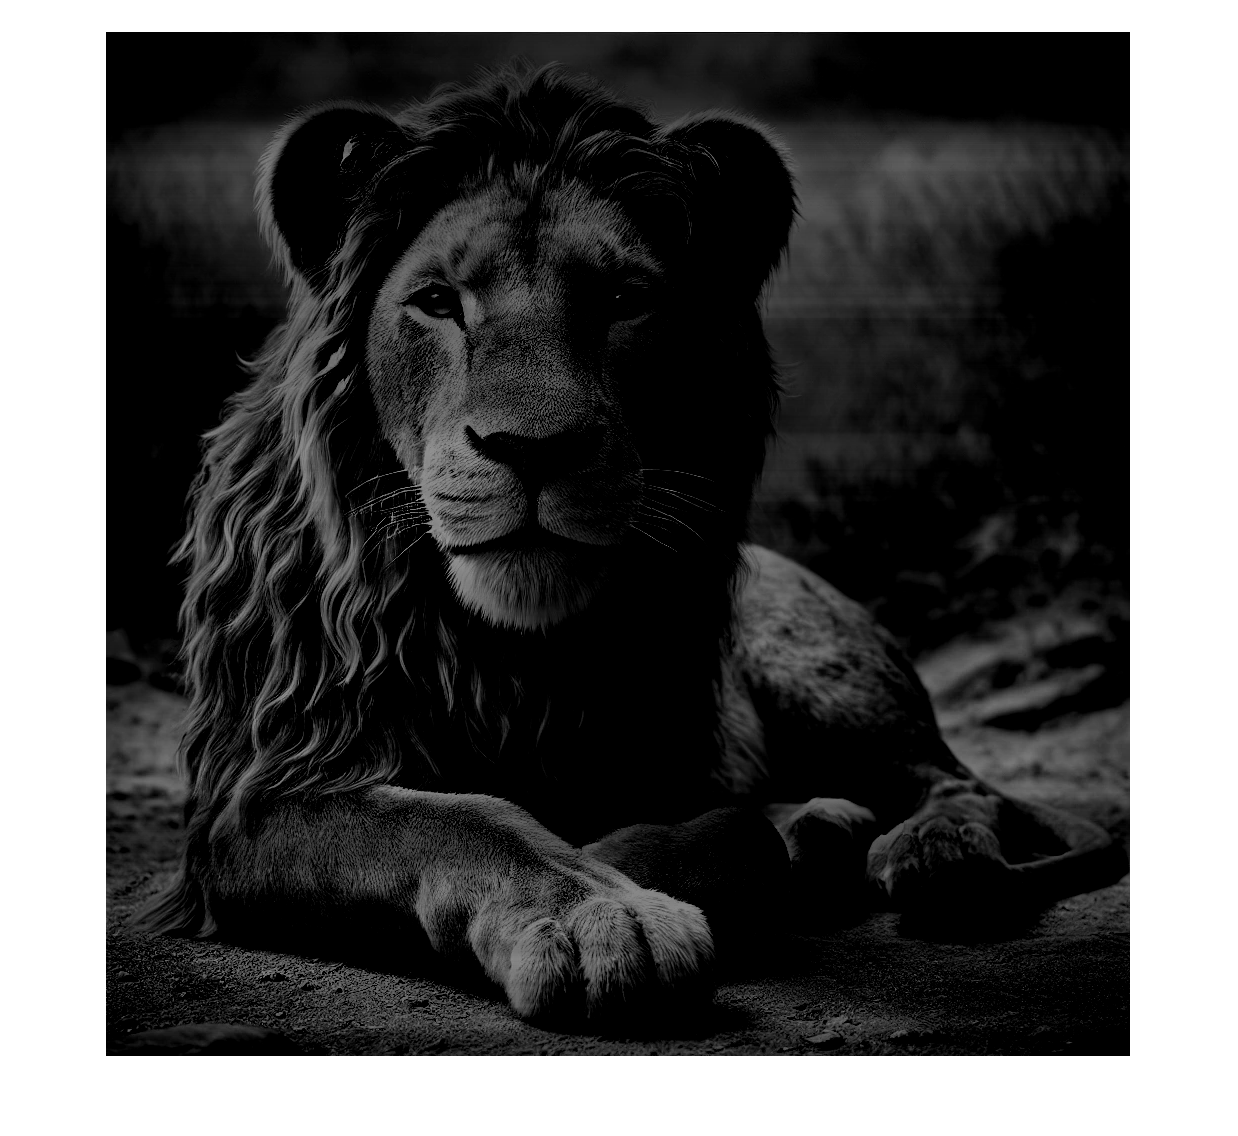
\includegraphics[width=22.62cm, height=20.76cm]{realistic_lion_centered.png}

\end{center}

The SVD of the centered lion gives $U$, $S$, and $V$ as $1024\times 1024$ matrices, meaning we have $1024$ possible principal components to work wtih. 

Reconstructing only on the $100$-dimensional best-fit subspace yields the following:

\begin{center}

  
\includegraphics[width=22.62cm, height=20.76cm]{realistic_lion_100_vals.png}

\end{center}

What is the difference between the total squared spread on the $100$-dimensional approximation and the total squared spread of the data on the remaining $924$ principal components? 

Answer in scientific notation:

$\answer{2.9}\times 10^{\answer{9}}$ (Round the coefficient to one decimal place.)

\end{problem}


\end{document}